% Repeated Labels. Slides 17 to 22.
\section{Repeated Labels}

% Source. Experiments 5.1.1, sec:exp-setup. CIFAR-10H image and counts.
% Delivery. Introduce the CIFAR-10H image. These are observed human labels, not a model illustration.
% Delivery. Retaining these labels preserves information that one selected label hides.
% Preparation. Do not assign this observed disagreement to a validated uncertainty component.
\begin{frame}{Repeated labels reveal disagreement}
\label{frm:observed-disagreement}
\slidemessage{Retaining repeated labels preserves observed disagreement.}
\begin{columns}[T,onlytextwidth]
\begin{column}{0.28\textwidth}
\centering
\vspace{3mm}

\includegraphics[width=0.88\linewidth]{figures/cifar10h_example.png}
\par\smallskip
{\small One CIFAR-10H image}
\end{column}
\begin{column}{0.70\textwidth}
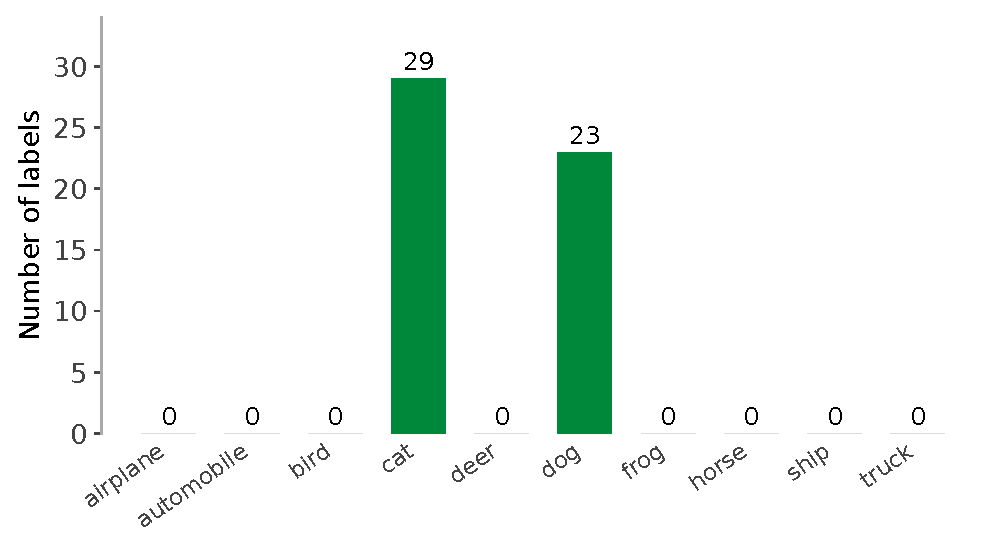
\includegraphics[width=\linewidth]{figures/observed_counts.pdf}
\end{column}
\end{columns}
\par\medskip
\slidepoint{\exampletotal{} observed human labels for the same input.}
% Preparation. \exampletotal{} human labels. The counts describe how labels differ for one input.
% Source detail. Thesis \S5.1.1. CIFAR-10H image \exampleindex{}.
\end{frame}

% Source. Methods 4.4.1 and 4.4.2, eq:mbnn-observation, eq:dm-ebnn-likelihood.
% Delivery. Both models use the same count vectors. Their observation models differ.
\begin{frame}{A model for complete count vectors}
\label{frm:count-model}
\slidemessage{Repeated labels change the observation model.}
\begin{itemize}
\item Labels are aggregated by class into a count vector $n$.
\begin{itemize}
\item The count total is $R=\sum_c n_c$.
\end{itemize}
\end{itemize}
\medskip
{\small Multinomial Bayesian neural network (M-BNN)}
% Copied from thesis eq:mbnn-observation.
\[
p(n\mid x,w)=\mathrm{Mult}\bigl(n\mid R,f(x;w)\bigr).
\]
{\small Dirichlet multinomial evidential Bayesian neural network (DM-eBNN)}
% Copied from thesis eq:dm-ebnn-likelihood.
\[
p(n\mid x,w)=\mathrm{DM}\bigl(n\mid R,\alpha(x;w)\bigr).
\]
\par\medskip
\slidepoint{$f(x;w)$ is the class-probability vector of the M-BNN.}
% Preparation. Both models use a posterior over shared weights. The DM-eBNN retains its Gamma prior.
% Source detail. Thesis \S4.4.1 and \S4.4.2.
\end{frame}

% Source. Methods 4.4.3 and 4.4.4, eq:dm-ebnn-posterior-odds, eq:count-variance-ratio.
% Figure comes from Background eq:multinomial-mass and eq:dm-mass.
% Delivery. State the fixed mean and count total before comparing the spread.
\begin{frame}{Count variance}
\label{frm:count-variance}
\slidemessage{The count likelihood can inform the total concentration parameter.}
\begin{center}
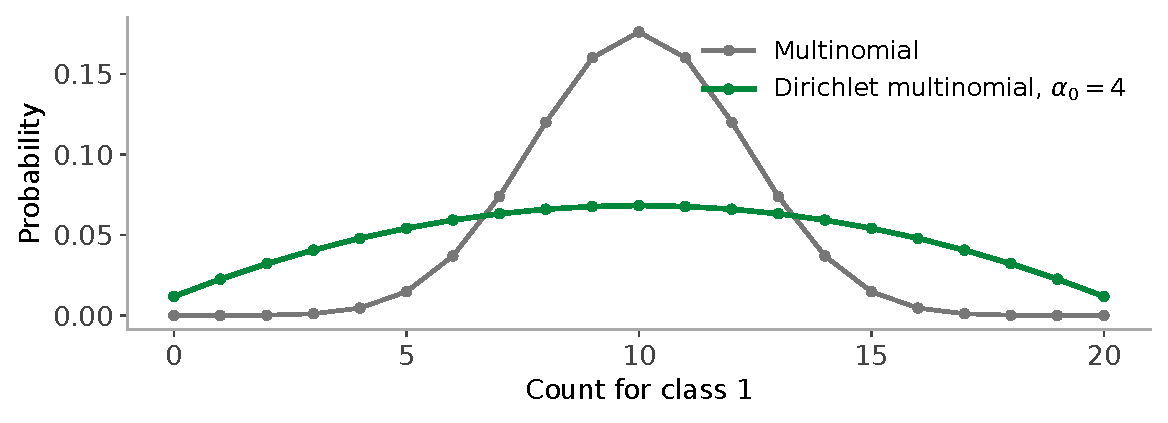
\includegraphics[width=0.90\textwidth]{figures/count_variance.pdf}
\end{center}
\begin{itemize}
\item The mean vector and count total stay fixed. The count probabilities differ.
\begin{itemize}
\item Two class illustration with mean vector $(0.5,0.5)$ and count total 20.
\end{itemize}
\end{itemize}
% Preparation. Mathematical illustration with two classes, mean vector $(0.5,0.5)$, and count total 20.\par
% At fixed mean vectors, this dependence on total concentration requires a count total above one.
% Source detail. Thesis \S4.4.3 and \S4.4.4.
\end{frame}

% Source. Experiments 5.3.1, tab:e2-count-prediction. All four comparisons are shown.
% Delivery. Explain the mean matched control before discussing the values.
\begin{frame}{Better count prediction on CIFAR-10H}
\label{frm:count-prediction}
\slidemessage{Additional count variance contributes to better count prediction.}
\begin{itemize}
\item The mean matched control keeps the DM-eBNN mean vectors and weight samples.
\begin{itemize}
\item Only the observation model changes to the multinomial distribution.
\end{itemize}
\end{itemize}
\begin{center}
\small
\renewcommand{\arraystretch}{1.12}
\setlength{\tabcolsep}{6pt}
% Generated by scripts/build_figures.py from unchanged thesis analysis outputs.
\begin{tabular}{lcccc}
\toprule
initialisation & \shortstack{Gamma prior\\mode} & \shortstack{M-BNN\\count NLL} & \shortstack{DM-eBNN\\count NLL} & \shortstack{mean matched\\control NLL} \\
\midrule
cold & 50 & \shortstack{19.161\\(18.012--19.754)} & \shortstack{12.718\\(12.486--13.007)} & \shortstack{23.719\\(23.195--24.467)} \\
cold & 200 & \shortstack{19.161\\(18.012--19.754)} & \shortstack{13.199\\(11.872--14.051)} & \shortstack{20.291\\(17.602--22.035)} \\
warm & 50 & \shortstack{27.540\\(23.630--31.685)} & \shortstack{14.392\\(13.724--15.529)} & \shortstack{28.802\\(26.771--32.415)} \\
warm & 200 & \shortstack{27.540\\(23.630--31.685)} & \shortstack{16.152\\(15.664--16.860)} & \shortstack{26.207\\(25.281--27.394)} \\
\bottomrule
\end{tabular}

\end{center}
\slidepoint{CIFAR-10H. Means and ranges over three seeds. Lower count NLL is better.}
% Preparation. Count negative log likelihood (count NLL). Lower is better. Points show means over three seeds. Bars show seed ranges.\par
% CIFAR-10H test split. Final BMA over 40 samples. DM-eBNN prior standard deviation 20\%.
% Source detail. Thesis \S5.3.1. Cold and warm chains have different sampling budgets.
\end{frame}

% Source. Experiments 5.3.2, tab:e2-count-prior-sensitivity.
% Delivery. The two trajectories approach each other but remain different within the budget.
\begin{frame}{Prior sensitivity remains}
\label{frm:count-prior-sensitivity}
\slidemessage{The prior and initial checkpoint still affect realised total concentration.}
\slidepoint{Realised total concentration after sampling on CIFAR-10H.}
\begin{center}
\renewcommand{\arraystretch}{1.65}
% Generated by scripts/build_count_sensitivity_table.py from unchanged thesis and analysis tables.
\begin{tabular}{ccccc}
\toprule
\shortstack{Pretraining\\prior mode} & \shortstack{SGLD prior SD\\(\% of mode)} & \shortstack{Realised total\\concentration} & \shortstack{Majority label\\accuracy} & \shortstack{Count NLL\\$\downarrow$ better} \\
\midrule
\shortstack{None\\(cold)} & No Gamma prior & 10.0\,(10.0--10.0) & 0.099\,(0.098--0.100) & 23.433\,(23.433--23.433) \\
\midrule
50 & 20\% & 51.0\,(50.8--51.1) & 0.753\,(0.720--0.777) & 14.392\,(13.724--15.529) \\
50 & 100\% & 69.8\,(69.2--70.3) & 0.754\,(0.723--0.776) & 13.626\,(12.863--14.940) \\
50 & No Gamma prior & 79.3\,(78.2--80.1) & 0.752\,(0.724--0.776) & 13.657\,(12.863--15.032) \\
\midrule
200 & 20\% & 182.7\,(181.5--184.8) & 0.773\,(0.759--0.781) & 16.152\,(15.664--16.860) \\
200 & 100\% & 162.5\,(160.6--165.5) & 0.771\,(0.758--0.781) & 14.439\,(13.983--15.153) \\
200 & No Gamma prior & 155.9\,(154.1--159.0) & 0.772\,(0.760--0.784) & 13.941\,(13.557--14.574) \\
\bottomrule
\end{tabular}

\end{center}
\slidepoint{Means and ranges over three seeds. Warm initialisation with a fixed sampling budget.}
% Preparation. Warm initialisation on CIFAR-10H. Mean and range over three seeds. Final BMA over 40 samples.\par
% Pretraining uses a Gamma prior standard deviation of 20\%. These results concern the fixed sampling budget.
% Source detail. Thesis \S5.3.2.
\end{frame}

% Source. Methods 4.4.5 and Experiments 5.3.3, sec:count-uncertainty-decomposition, tab:e2-count-terms.
% Delivery. These are terms for one class label, although training uses count vectors.
\begin{frame}{Decomposition for class labels}
\label{frm:count-decomposition}
\slidemessage{The DM-eBNN reports the three terms. Their practical value remains open.}
\begin{center}
\renewcommand{\arraystretch}{1.6}
\setlength{\tabcolsep}{7pt}
% Generated by scripts/build_figures.py from unchanged thesis analysis outputs.
\begin{tabular}{lcccc}
\toprule
model & \shortstack{Gamma prior\\mode} & \shortstack{aleatoric\\uncertainty \%} & \shortstack{distributional\\uncertainty \%} & \shortstack{epistemic\\uncertainty \%} \\
\midrule
M-BNN & -- & 95.25 & -- & 4.75 \\
DM-eBNN & 50 & 87.60 & 7.71 & 4.69 \\
DM-eBNN & 200 & 88.28 & 4.07 & 7.65 \\
\bottomrule
\end{tabular}

\end{center}
\begin{itemize}
\item Shares of each model's own predictive uncertainty in a class label.
\begin{itemize}
\item CIFAR-10H. Averages over inputs and three seeds. Warm initialisation.
\end{itemize}
\end{itemize}
% Preparation. Shares of each model's own predictive uncertainty, averaged over inputs and three seeds.\par
% CIFAR-10H test split. Warm initialisation. Final BMA over 40 samples. DM-eBNN prior standard deviation 20\%.
% Source detail. Thesis \S4.4.5 and \S5.3.3.
\end{frame}
